\begin{example} \label{eg:6.1.1} % EXAMPLE
Find the volume of the solid of revolution generated when the region $R$ bounded by $y = 4-x^2$ and the $x$-axis is revolved about the $x$-axis.

\solution
First, we observe that $y = 4-x^2$ intersects the $x$-axis at the points $(-2,0)$ and $(2,0)$.  When we take the region $R$  that lies between the curve and the $x$-axis on this interval and revolve it about the $x$-axis, we get the three-dimensional solid pictured in Figure~\ref{F:6.1.Ex1}.

Taking a representative slice of the solid located at a value $x$ that lies between $x = -2$ and $x = 2$, we see that the thickness of such a slice is $\triangle x$ (which is also the height of the cylinder-shaped slice), and that the radius of the slice is determined by the curve $y = 4-x^2$.  Hence, we find that 
$$V_{\text{\small{slice}}} = \pi (4-x^2)^2 \triangle x,$$
since the volume of a cylinder of radius $r$ and height $h$ is $V = \pi r^2 h$.

Using a definite integral to sum the volumes of the representative slices, it follows that 
$$V = \int_{-2}^{2} \pi (4-x^2)^2 \, dx.$$
It is straightforward to evaluate the integral and find that the volume is $V = \frac{512}{15}\pi$.	
\end{example}

\begin{marginfigure}[-8cm] %MARGIN FIGURE
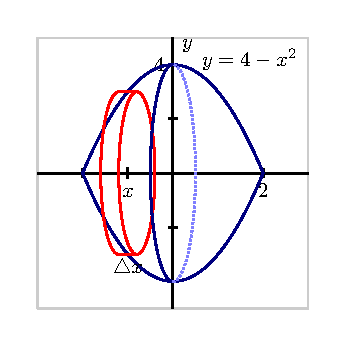
\includegraphics{figures/6_2_Ex1.eps}
\caption{The solid of revolution in Example~\ref{eg:6.1.1}.} \label{F:6.1.Ex1}
\end{marginfigure}

